
\section{Evaluation}
\label{sec:evaluation}

This section is organized into four subsections: (1) Data, (2) CoAtNets vs VTs, (3) Mitigating errors with LLMs, and (4) Mitigating errors with fine-tuned LLMs.

\subsection{Dataset}

The original keystroke dataset consists of two datasets, which are from the noise-free Phone and Zoom recordings with lacked space characters. To simulate real-world sentences, we assumed spaces existed in the dataset with the same prediction accuracy as other letters and digits. To evaluate error detection and correction, the EnglishTense dataset~\cite{ayman2024englishtense} was used, which contains a rich corpus of categorized English sentences. From this dataset, 1,000 sentences were randomly selected: 500 containing digits and 500 without digits, ensuring a balanced variety of sentence structures and types.
\par
\begin{table}[htbp]
\centering
\resizebox{\columnwidth}{!}{%
\begin{tabular}{l|ccc}
    \toprule
    \textbf{Dataset name / Noise Factor ($\eta$)} & \textbf{Low} & \textbf{Medium} & \textbf{High} \\ \midrule
    Phone            & 0.012            & 0.024             & 0.06             \\ 
    Zoom             & 0.1            & 0.5               & 1.0             \\ 
    \bottomrule
\end{tabular}%
}
\vspace{0.2em}
\caption{Different noise intensity levels across Phone and Zoom datasets.}
\label{tab:noise_factors}
\end{table}
\par

We utilized the same datasets as in ~\cite{harrison2023practical}. The data were collected from two sources: Phone and Zoom ~\cite{datasetgithublink}, which contain recordings of 36 distinct keystrokes (letters a–z and digits 0–9), with each keystroke recorded 25 times using either setup. 
In the Phone setup, the sound of a victim’s laptop keystrokes was recorded using an iPhone (representing the attacker). In the Zoom setup, the victim’s laptop keystroke sounds were captured via Zoom's built-in recording function, with the audio obtained from the victim’s microphone.
We selected this dataset over other available options for several reasons: (1) It is a recent dataset (2023) specifically designed for acoustic side-channel attacks; (2) it employs recordings from a widely available, modern laptop, the MacBook Pro 16-inch (2021), whose keyboard design remains prevalent in current (2025) MacBook models; and (3) the Zoom recording setup offers a particularly realistic scenario, given the widespread use of Zoom today. 
\par 
However, a significant limitation of this dataset is that all recordings were made in a noise-free environment. Consequently, it does not fully reflect real-world scenarios, and a standalone classification model is likely to struggle when confronted with even minimal background noise, a challenge we address using an LLM-based correction mechanism. Additionally, the dataset does not include \textit{space}, \textit{backspace}, and \textit{enter} keystrokes, which are essential components of typical keyboard usage. We discuss these issues in more detail in Section~\ref{sec:discussion}.
\par 
Since each keystroke was recorded 25 times consecutively, every audio file was segmented into 25 individual \textit{.wav} files. To achieve this, we first applied a Fast Fourier Transform (FFT) to each recording and summed the frequency coefficients to compute the energy. This energy measure allowed us to identify 25 distinct peaks per keystroke, thereby dividing the audio into 25 separate files per key, resulting in a total of 900 samples. We followed the step shown in Fig.~\ref{fig:data_processing} to generate mel-spectrogram images. 
\par 
The input image dimensions vary between models: CoAtNet utilizes 64$\times$64 images, while VT models require 224$\times$224 images. We employed the Adam~\cite{kingma2014adam} optimizer for CoAtNet and AdamW~\cite{loshchilov2017decoupled} for VT models. Table~\ref{tab:keystroke_hyperparameters} provides detailed hyperparameters used throughout our experiments, from image generation to testing. To compare the performance of CoAtNet and VT models, we applied two distinct data transformation methods to the VT inputs. These methodologies enable a comprehensive evaluation under different preprocessing conditions:
\begin{enumerate}[label=(\arabic*)]
    \item \textbf{Resizing Transformation:} Input images initially sized at 64$\times$64 were resized using bilinear interpolation to 224$\times$224 to meet the VT models' requirements. 
    % The images were then normalized, and random erasing was applied as a data augmentation technique.
    \item \textbf{Direct Transformation:} By modifying the hyperparameters of the mel-spectrogram generation process, input images were directly produced at a resolution of 224$\times$224, thereby eliminating the need for resizing. 
    % In this case, normalization and time-frequency masking were employed for data augmentation.
\end{enumerate}
\begin{table}[htbp]
    \centering
    \resizebox{\columnwidth}{!}{%
    \begin{tabular}{l|cc}
        \toprule
         & \textbf{Phone Value} & \textbf{Zoom Value} \\ \midrule
        Epochs      & 1100 & 1100 \\
        Batch Size  & 16 & 16 \\
        Loss Type   & Cross Entropy & Cross Entropy \\
        Optimizer   & Adam$^*$ / AdamW$^\dagger$ & Adam$^*$ / AdamW$^\dagger$ \\
        Max Learning Rate        & 5e-4$^*$ / 5e-5$^\dagger$ & 5e-4$^*$ / 5e-5$^\dagger$\\
        Annealing Schedule       & Linear & Linear \\
        Timeshift Percentage     & 0.3 & 0.4 \\
        Max Mask Percentage      & 0.1 $^*$ / 0.03$^\dagger$ & 0.1 $^*$ / 0.03$^\dagger$\\
        Number of Masks Per Axis & 2 & 2 \\
        Mel Bands       & 64$^*$ / 224$^\dagger$ & 64$^*$ / 224$^\dagger$\\
        FFT Window Size & 1024 & 1024 \\
        Hop Length      & 300$^*$ / 85$^\dagger$ & 226$^*$ / 64$^\dagger$\\
        Data Split      & Stratified & Stratified\\
        \bottomrule
    \end{tabular}%
    }
    \vspace{0.2em}
    \caption{Hyperparameters for keystroke classification experiments using Phone and Zoom recordings. $^*$ indicates values used in our CoAtNet implementation, while $^\dagger$ indicates values used in the selected VT models}
    \label{tab:keystroke_hyperparameters}
\end{table}

\subsection{Metrics}
The corrected sentences were evaluated using multiple metrics to quantify performance:
\begin{itemize}
    \item \textbf{BLEU:} Measures n-gram overlap between the corrected sentence and the ground truth.
    \item \textbf{ROUGE:} Evaluates recall-based overlap of substrings.
    \item \textbf{METEOR:} Considers synonymy and stemming in evaluating similarity.
\end{itemize}

\subsection{Research Questions (RQs)}

\begin{enumerate}
    \item How do the different Visual Transformer (VT) architectures perform in acoustic keystroke classification compared to the state-of-the-art baseline CoAtNet under ideal (noise-free) conditions?
    \item Can Large Language Models (LLMs), such as GPT-4o and Llama models, effectively correct errors in keystroke predictions resulting from realistic acoustic noise?
    \item How does fine-tuning smaller LLMs using Low-Rank Adaptation (LoRA) affect their performance in error correction compared to larger LLMs like GPT-4o in acoustic side-channel attacks?
\end{enumerate}

\subsection{RQ1: CoAtNets vs VTs}
Using the details outlined in the methodology section, we compared B-CoAtNet with our CoAtNet (we will now refer to it as O-CoAtNet for our CoAtNet) using a noise-free dataset. As shown in Table \ref{tab:coatnet}, O-CoAtNet achieves higher accuracy than B-CoAtNet in terms of both mean and standard deviation, as well as maximum accuracy.
For the Phone dataset, we observe a 1.5\% increase in mean accuracy, while for the Zoom dataset, the improvement is 3.5\%. Given that the original work reported only the best accuracy without providing a mean or standard deviation, the gap between the best accuracy of B-CoAtNet and O-CoAtNet is even more significant. We show a 5.0\% increase in the Phone dataset, while for the Zoom dataset, the improvement is 5.9\%.
Given that we utilized the lightweight CoAtNet model, we anticipate that even higher accuracy could be achieved with a heavyweight CoAtNet model, as previous work ~\cite{dai2021coatnet} reports better performance for heavyweight CoAtNet configurations under ImageNet ~\cite{5206848} and JFT-300M ~\cite{sun2017revisiting} datasets.
\begin{table}[htbp]
    \centering
    \resizebox{\columnwidth}{!}{%
    \begin{tabular}{l|cc}
        \toprule
        & \textbf{B-CoAtNet (Unknown)} & \textbf{O-CoAtNet ($\sim$24M)} \\ \midrule
        Phone: Mean and stdev & - & 96.45 $\pm$ 3.5\% \\
        Phone: Max  & 95\% & \textbf{100\%} \\
        \midrule
        Zoom: Mean and stdev & - & 96.67 $\pm$ 2.1\% \\
        Zoom: Max  & 93\% & \textbf{98.9\%} \\
        \bottomrule
    \end{tabular}%
    }
    \vspace{0.2em}
    \caption{Summary statistics for B-CoAtNet vs O-CoAtNet on the noise-free Phone and Zoom datasets. For our CoAtNet, the mean and standard deviation were calculated based on results from five different seeds. Note that B-CoAtNet only reports the best accuracy without providing standard deviations or parameter sizes, the latter of which is marked as `unknown' in the table.}
    \label{tab:coatnet}
\end{table}
\par
We also compared B-CoAtNet with selected VTs, including a reference to the number of parameters for each model. By examining the results in Tables \ref{tab:trans1}, we observe that VTs demonstrate comparable or, in some cases, superior accuracy to B-CoAtNet. 
When comparing the best accuracy between B-CoAtNet and selected VTs, the direct transformation using Swin exhibits the largest gap, with a 5.0\% difference on the Phone dataset and a 5.9\% difference on the Zoom dataset.
Considering other models, they also demonstrate accuracy comparable to B-CoAtNet. 
However, the CLIP model exhibits significantly lower performance. We suspect this is due to CLIP being originally designed for multimodal tasks, while we utilized only its vision component. Here we want to note that, we did not fine-tune hyperparameters of VTs such as the learning rate, batch size, or scheduler, which likely contributed to the weaker performance. We strongly believe that performance could be improved through hyperparameter optimization.
\begin{table*}[htbp]
    \centering
    \small
    % Define uniform column widths using p{}
    \begin{tabular}{p{4cm}|p{2.25cm}p{2.25cm}p{2.25cm}p{2.25cm}p{2.25cm}}
        \toprule
        \textbf{Resizing Transformation} & \textbf{ViT (86M)} & \textbf{Swin (28M)} & \textbf{DeiT (86M)} & \textbf{CLIP (87M)} & \textbf{BEiT (86M)} \\ 
        \midrule
        Phone: Mean and stdev & 94.8\% $\pm$ 1.0\% & 90.0\% $\pm$ 7.6\% & 89.3\% $\pm$ 3.3\% & 76.9\% $\pm$ 3.8\% & \textbf{95.6\% $\pm$ 1.4\%} \\
        Phone: Max & 95.6\% & \textbf{98.9\%} & 92.2\% & 81.1\% & 97.8\% \\
        \midrule
        Zoom: Mean and stdev & \textbf{90.4\% $\pm$ 3.0\%*} & 85.1\% $\pm$ 3.4\% & 85.3\% $\pm$ 2.0\% & 66.2\% $\pm$ 8.9\% & 87.1\% $\pm$ 4.1\% \\
        Zoom: Max & \textbf{94.4\%} & 88.9\% & 87.8\% & 78.9\% & 92.2\% \\ 
        \bottomrule
        \noalign{\vspace{1.0em}} % Adds vertical space within the tabular
    % \end{tabular}
    % \begin{tabular}{p{4cm}|p{2.25cm}p{2.25cm}p{2.25cm}p{2.25cm}p{2.25cm}}
        \toprule
        \textbf{Direct Transformation} & \textbf{ViT (86M)} & \textbf{Swin (28M)} & \textbf{DeiT (86M)} & \textbf{CLIP (87M)} & \textbf{BEiT (86M)} \\ 
        \midrule
        Phone: Mean and stdev & 94.0\% $\pm$ 2.3\% & 96.7\% $\pm$ 2.5\% & 94.4\% $\pm$ 1.4\% & 84.9\% $\pm$ 6.7\% & \textbf{97.6\% $\pm$ 1.6\%*} \\
        Phone: Max & 97.8\% & \textbf{100.0\%*} & 95.6\% & 90.0\% & \textbf{100.0\%*} \\
        \midrule
        Zoom: Mean and stdev & 56.4\% $\pm$ 48.8\% & 54.7\% $\pm$ 48.4\% & 22.2\% $\pm$ 40.4\% & 2.7\% $\pm$ 0.6\% & \textbf{57.3\% $\pm$ 45.9\%} \\
        Zoom: Max & 95.6\% & \textbf{98.9\%*} & 94.4\% & 3.3\% & 96.7\% \\
        \bottomrule
    \end{tabular}
    \vspace{0.2em}
    \caption{Summary statistics for different transformer models on the Phone and Zoom dataset using resizing transformation and direct transformation. The mean and standard deviation (stdev) were calculated using results from five different seeds. Bolded numbers indicate the best performance in each row, while an asterisk (*) denotes the best for each dataset.}
    \label{tab:trans1}
\end{table*}
\par
When evaluating the number of parameters, VTs do not appear to offer a clear performance advantage over CoAtNet, as they have a much larger parameter count. This is likely due to the limited size of the dataset, which contains only 25 samples per syllable or digit. We presume that collecting a larger dataset or employing additional data augmentation techniques could improve accuracy in VTs. Overall, our results show that VTs can perform on par with or even exceed CoAtNet. 
\par
Importantly, our goal was not merely to achieve better performance using VTs, but to assess their potential as alternative models for acoustic SCA keystroke classification. We are primarily focused on enhancing the performance of the ASCA keystroke classification task, especially under realistic conditions where environmental noise is inevitable. To address this challenge, we introduce a LLM to complement the classification process. Recognizing that relying solely on refined datasets can be impractical in noisy environments, our approach aims to improve robustness and accuracy. In the following subsection, we demonstrate how LLMs can be effectively leveraged to mitigate noise-related issues, thereby addressing more realistic operational conditions.

\subsection{RQ2: Mitigating errors with LLMs}
We present the experimental results demonstrating the performance of various LLM models in correcting noisy text predictions across multiple noise levels. 
The evaluation utilized multiple metrics, including BLEU, METEOR, and ROUGE scores, providing a comprehensive analysis of the effectiveness of LLMs in improving the robustness of ASCAs. 
We evaluated the error mitigation capabilities of LLM models, specifically the Llama family and GPT-4o, by varying error rates and performance metrics. 
\par 
\begin{table*}[htbp]
    \centering
    \small
    \begin{tabular}{l|p{2cm}p{2cm}p{2cm}p{2cm}p{2cm}p{2cm}}
        \toprule
        \textbf{Metric (Noise Factor)} & \textbf{B-CoAtNet} & \textbf{Llama-3.2-1B} & \textbf{Llama-3.2-3B} & \textbf{Llama-3.1-8B} & \textbf{GPT-4o ($\sim$200B)} &\textbf{Llama-3.2-3B (Fine-tuned)} \\ \midrule
        % phone ds
        BLEU (Low) & 0.383 $\pm$ 0.249 & 0.684 $\pm$ 0.294 & 0.863 $\pm$ 0.183 & 0.910 $\pm$ 0.159 & 0.975 $\pm$ 0.075* & \textbf{0.977 $\pm$ 0.073} \\
        BLEU (Mid) & 0.078 $\pm$ 0.091 & 0.273 $\pm$ 0.268 & 0.542 $\pm$ 0.282 & 0.681 $\pm$ 0.258 & \textbf{0.916 $\pm$ 0.120} & 0.908 $\pm$ 0.156* \\
        BLEU (High) & 0.021 $\pm$ 0.023 & 0.041 $\pm$ 0.083 & 0.118 $\pm$ 0.151 & 0.189 $\pm$ 0.196 & \textbf{0.638 $\pm$ 0.287} & 0.623 $\pm$ 0.302* \\
        \midrule
        Meteor (Low) & 0.640 $\pm$ 0.190 & 0.830 $\pm$ 0.213 & 0.941 $\pm$ 0.084 & 0.964 $\pm$ 0.070 & 0.988 $\pm$ 0.032* & \textbf{0.990 $\pm$ 0.032} \\
        Meteor (Mid) & 0.286 $\pm$ 0.162 & 0.504 $\pm$ 0.273 & 0.751 $\pm$ 0.184 & 0.846 $\pm$ 0.143 & 0.958 $\pm$ 0.057* & \textbf{0.960 $\pm$ 0.073} \\
        Meteor (High) & 0.082 $\pm$ 0.085 & 0.137 $\pm$ 0.159 & 0.344 $\pm$ 0.211 & 0.454 $\pm$ 0.219 & 0.804 $\pm$ 0.189* & \textbf{0.807 $\pm$ 0.191} \\
        \midrule
        Rouge-1 (Low) & 0.690 $\pm$ 0.157 & 0.844 $\pm$ 0.194 & 0.944 $\pm$ 0.080 & 0.964 $\pm$ 0.071 & 0.989 $\pm$ 0.032* & \textbf{0.990 $\pm$ 0.034} \\
        Rouge-1 (Mid) & 0.374 $\pm$ 0.148 & 0.552 $\pm$ 0.249 & 0.777 $\pm$ 0.159 & 0.856 $\pm$ 0.129 & \textbf{0.960 $\pm$ 0.055} & \textbf{0.960 $\pm$ 0.071} \\
        Rouge-1 (High) & 0.141 $\pm$ 0.113 & 0.196 $\pm$ 0.173 & 0.406 $\pm$ 0.196 & 0.503 $\pm$ 0.200 & \textbf{0.817 $\pm$ 0.171} & 0.815 $\pm$ 0.176* \\
        \midrule
        Rouge-2 (Low) & 0.497 $\pm$ 0.226 & 0.754 $\pm$ 0.251 & 0.899 $\pm$ 0.137 & 0.932 $\pm$ 0.121 & 0.979 $\pm$ 0.061* & \textbf{0.982 $\pm$ 0.060} \\
        Rouge-2 (Mid) & 0.131 $\pm$ 0.136 & 0.361 $\pm$ 0.276 & 0.629 $\pm$ 0.240 & 0.748 $\pm$ 0.209 & 0.925 $\pm$ 0.103* & \textbf{0.927 $\pm$ 0.123} \\
        Rouge-2 (High) & 0.017 $\pm$ 0.050 & 0.059 $\pm$ 0.122 & 0.191 $\pm$ 0.190 & 0.285 $\pm$ 0.214 & \textbf{0.703 $\pm$ 0.244} & 0.701 $\pm$ 0.254* \\
        \midrule
        Rouge-L (Low) & 0.690 $\pm$ 0.157 & 0.844 $\pm$ 0.194 & 0.943 $\pm$ 0.080 & 0.963 $\pm$ 0.073 & 0.989 $\pm$ 0.032* & \textbf{0.990 $\pm$ 0.034} \\
        Rouge-L (Mid) & 0.374 $\pm$ 0.148 & 0.550 $\pm$ 0.249 & 0.776 $\pm$ 0.160 & 0.856 $\pm$ 0.130 & \textbf{0.960 $\pm$ 0.055} & \textbf{0.960 $\pm$ 0.071} \\
        Rouge-L (High) & 0.141 $\pm$ 0.113 & 0.194 $\pm$ 0.172 & 0.400 $\pm$ 0.196 & 0.497 $\pm$ 0.202 & \textbf{0.816 $\pm$ 0.172} & 0.814 $\pm$ 0.179* \\
        \bottomrule
    \end{tabular}
    \vspace{0.2em}
    \caption{Performance using metrics -- BLEU, METEOR, ROUGE-1, ROUGE-2, and ROUGE-L -- for different models at varying noise factors on the Phone dataset. Bolded numbers indicate the best performance (mean) in each row, while an asterisk (*) shows the second-best performance (mean) within the same metric.}
    \label{tab:metrics_noise_levels_phone}
\end{table*}
\begin{table*}[htbp]
    \centering
    \small
    \begin{tabular}{l|p{2cm}p{2cm}p{2cm}p{2cm}p{2cm}p{2cm}}
        \toprule
        \textbf{Metric (Noise Factor)} & \textbf{B-CoAtNet} & \textbf{Llama-3.2-1B} & \textbf{Llama-3.2-3B} & \textbf{Llama-3.1-8B} & \textbf{GPT-4o ($\sim$200B)} & \textbf{Llama-3.2-3B (Fine-tuned)} \\ \midrule
        % zoom ds
        BLEU (Low) & 0.285 $\pm$ 0.218 & 0.657 $\pm$ 0.297 & 0.827 $\pm$ 0.211 & 0.891 $\pm$ 0.167 & \textbf{0.976 $\pm$ 0.070} & 0.955 $\pm$ 0.099* \\
        BLEU (Mid) & 0.050 $\pm$ 0.057 & 0.193 $\pm$ 0.225 & 0.385 $\pm$ 0.273 & 0.520 $\pm$ 0.288 & \textbf{0.896 $\pm$ 0.152} & 0.866 $\pm$ 0.184* \\
        BLEU (High) & 0.018 $\pm$ 0.022 & 0.025 $\pm$ 0.055 & 0.081 $\pm$ 0.126 & 0.107 $\pm$ 0.151 & \textbf{0.542 $\pm$ 0.303} & 0.489 $\pm$ 0.303* \\
        \midrule
        Meteor (Low) & 0.551 $\pm$ 0.191 & 0.811 $\pm$ 0.211 & 0.923 $\pm$ 0.101 & 0.952 $\pm$ 0.076 & \textbf{0.988 $\pm$ 0.031} & 0.979 $\pm$ 0.043* \\
        Meteor (Mid) & 0.210 $\pm$ 0.143 & 0.412 $\pm$ 0.261 & 0.646 $\pm$ 0.216 & 0.751 $\pm$ 0.186 & \textbf{0.950 $\pm$ 0.073} & 0.938 $\pm$ 0.088* \\
        Meteor (High) & 0.065 $\pm$ 0.076 & 0.085 $\pm$ 0.117 & 0.268 $\pm$ 0.191 & 0.319 $\pm$ 0.200 & \textbf{0.735 $\pm$ 0.218} & 0.710 $\pm$ 0.226* \\
        \midrule
        Rouge-1 (Low) & 0.608 $\pm$ 0.161 & 0.826 $\pm$ 0.190 & 0.927 $\pm$ 0.092 & 0.954 $\pm$ 0.070 & \textbf{0.989 $\pm$ 0.031} & 0.979 $\pm$ 0.042* \\
        Rouge-1 (Mid) & 0.291 $\pm$ 0.144 & 0.461 $\pm$ 0.241 & 0.676 $\pm$ 0.195 & 0.769 $\pm$ 0.168 & \textbf{0.952 $\pm$ 0.070} & 0.940 $\pm$ 0.085* \\
        Rouge-1 (High) & 0.111 $\pm$ 0.102 & 0.131 $\pm$ 0.137 & 0.329 $\pm$ 0.184 & 0.373 $\pm$ 0.188 & \textbf{0.750 $\pm$ 0.199} & 0.722 $\pm$ 0.208* \\
        \midrule
        Rouge-2 (Low) & 0.392 $\pm$ 0.212 & 0.726 $\pm$ 0.254 & 0.868 $\pm$ 0.159 & 0.915 $\pm$ 0.129 & \textbf{0.979 $\pm$ 0.060} & 0.962 $\pm$ 0.079* \\
        Rouge-2 (Mid) & 0.083 $\pm$ 0.103 & 0.276 $\pm$ 0.248 & 0.493 $\pm$ 0.252 & 0.622 $\pm$ 0.242 & \textbf{0.914 $\pm$ 0.121} & 0.891 $\pm$ 0.143* \\
        Rouge-2 (High) & 0.014 $\pm$ 0.044 & 0.031 $\pm$ 0.084 & 0.132 $\pm$ 0.162 & 0.172 $\pm$ 0.183 & \textbf{0.615 $\pm$ 0.268} & 0.572 $\pm$ 0.272* \\
        \midrule
        Rouge-L (Low) & 0.608 $\pm$ 0.161 & 0.826 $\pm$ 0.190 & 0.927 $\pm$ 0.092 & 0.953 $\pm$ 0.072 & \textbf{0.989 $\pm$ 0.031} & 0.979 $\pm$ 0.042* \\
        Rouge-L (Mid) & 0.291 $\pm$ 0.144 & 0.458 $\pm$ 0.241 & 0.673 $\pm$ 0.197 & 0.765 $\pm$ 0.172 & \textbf{0.952 $\pm$ 0.070} & 0.939 $\pm$ 0.085* \\
        Rouge-L (High) & 0.111 $\pm$ 0.102 & 0.130 $\pm$ 0.135 & 0.313 $\pm$ 0.186 & 0.364 $\pm$ 0.190 & \textbf{0.749 $\pm$ 0.200} & 0.720 $\pm$ 0.210* \\
        \bottomrule
    \end{tabular}
    \vspace{0.2em}
    \caption{Performance using metrics -- BLEU, METEOR, ROUGE-1, ROUGE-2, and ROUGE-L -- for different models at varying noise factors on the Zoom dataset. Bolded numbers indicate the best performance (mean) in each row, while an asterisk (*) shows the second-best performance (mean) within the same metric.}
    \label{tab:metrics_noise_levels_zoom}
\end{table*}
From Table~\ref{tab:metrics_noise_levels_phone} and \ref{tab:metrics_noise_levels_zoom}, it is evident that B-CoAtNet performs poorly in the presence of noise. Without error mitigation techniques, relying solely on a classification model is inadequate.  
This outcome aligns with our expectations and underscores the need for LLMs to effectively mitigate errors.
Here, we show that incorporating LLMs for error detection and correction significantly improves performance. 
Within the Llama family, performance improves with larger model sizes. Among all tested LLMs, GPT-4o achieves the best results, particularly excelling under high noise conditions. 
\par 
The results indicate that LLMs are highly effective in detecting and correcting errors caused by noise in ASCA applications. GPT-4o, in particular, emerged as the most robust model, maintaining high performance across all metrics and noise levels. These findings underscore the potential of LLMs to enhance real-world applications where environmental noise poses a significant challenge.
\par 
Although GPT-4o achieves the best performance across all metrics, its major drawback is the high number of parameters and the long inference time it requires. GPT-4o has 200$\times$, 67$\times$, 25$\times$ more parameters compared to Llama-3.2-1B, Llama-3.2-3B, and Llama-3.2-8B, respectively. In the next section, we demonstrate that comparable accuracy to GPT-4o can be achieved by fine-tuning a lightweight Llama model.

\subsection{RQ3: Mitigating errors with Fine-tuned LLMs}
\label{sec:ft_results}
Utilizing the same datasets as in the previous subsection, we fine-tuned the weights of Llama-3.2-3B and compared its performance with GPT-4o.
Similar to the previous analysis, we evaluated the performance using multiple metrics. See the rightmost column in Table~\ref{tab:metrics_noise_levels_phone} and \ref{tab:metrics_noise_levels_zoom}. Additionally, the results are visualized in Fig.~\ref{fig:rotated}. 
Both tables and graphs clearly demonstrate the fine-tuned model's strong ability to correct mistakes compared to other models. For the Phone dataset, the fine-tuned Llama outperforms GPT-4o when noise levels are moderate (Low and Mid). In contrast, for the Zoom dataset, GPT-4o consistently delivers superior performance under all conditions. Nonetheless, the fine-tuned model consistently ranks as the second-best performer.
\par
The fine-tuned model exhibits consistent performance improvements across all evaluation metrics. In comparison to the original Llama model without fine-tuning, the fine-tuned 3B model outperforms it by a significant margin. For instance, when performance gain is measured as the average percentage increase in BLEU accuracy across various noise levels, the fine-tuned 3B model shows nearly a 170\% improvement over the original 3B model for the Phone dataset. Moreover, it outperforms the larger 8B model by 90\%. A similar trend is observed on the Zoom dataset, with an 215\% improvement over the original 3B model and a 145\% increase compared to the 8B model. These results clearly demonstrate the substantial benefits of fine-tuning, enabling a smaller model to outperform even larger variants.
\par
The fine-tuning is especially effective at higher noise levels. For example, with the noise intensity set to High, the fine-tuning increased the BLEU accuracy by 430\% and 500\% on the phone and Zoom datasets, respectively, compared to the original 3B model 
Its effect is not as evident at Low noise intensity as they are already close to 1. 
Similar levels of improvement are observed in other metrics as well. 
For instance, in Fig.~\ref{fig:rotated}, the fine-tuned 3B model (in brown) performs considerably better than all the other Llama models (1B, 3B, 8B in orange, green, and red, respectively) under all evaluation metrics at higher noise settings. 
\par
Despite having only about 1.5\% of the parameter count of the much larger GPT-4o, the fine-tuned model delivers comparable performance, achieving at least 90\% of GPT-4o’s scores across all evaluation metrics.
Our fine-tuning aligns the small Llama model with the large GPT-4o model in terms of noise tolerance.
This indicates that a lightweight model like Llama-3.2-3B is sufficient to complete the error correction task.
In conclusion, we showed that the fine-tuning approach has proven to be highly effective, transforming the pipeline’s output from partially correct sentences to highly accurate predictions of the ground truth sentences.
\par

\begin{figure*}[t]
    \centering

    % phone
    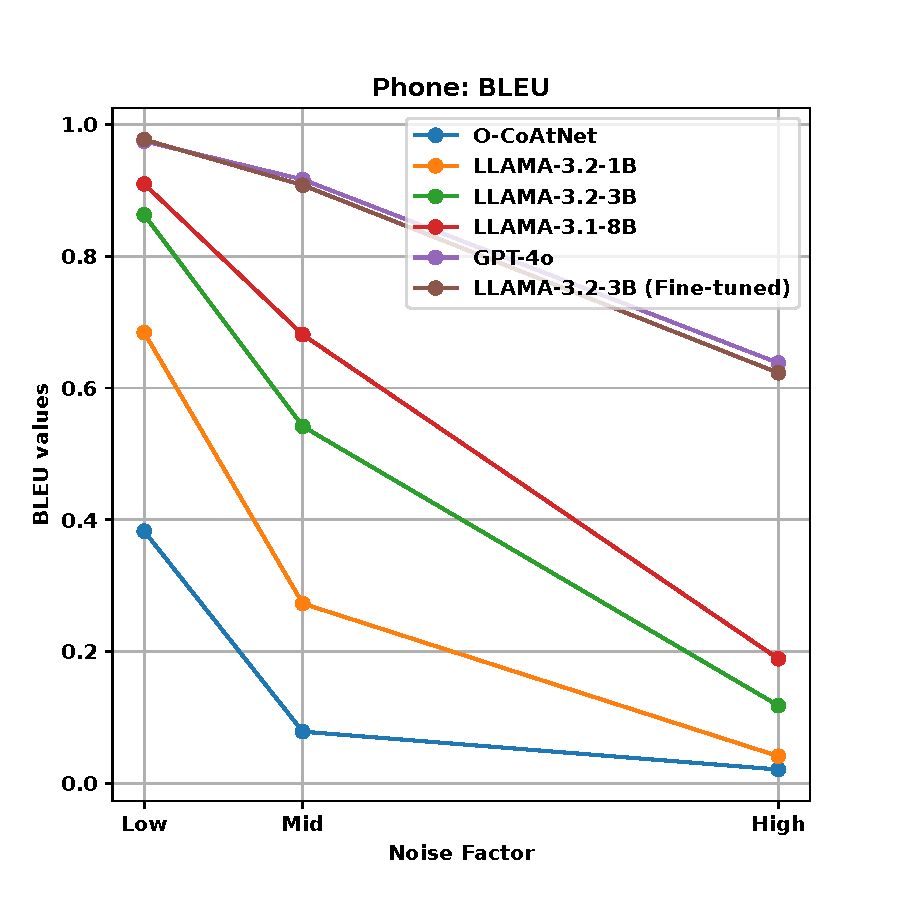
\includegraphics[width=0.20\textwidth]{images/BLEU_Accuracy_phone.pdf}\hfill
    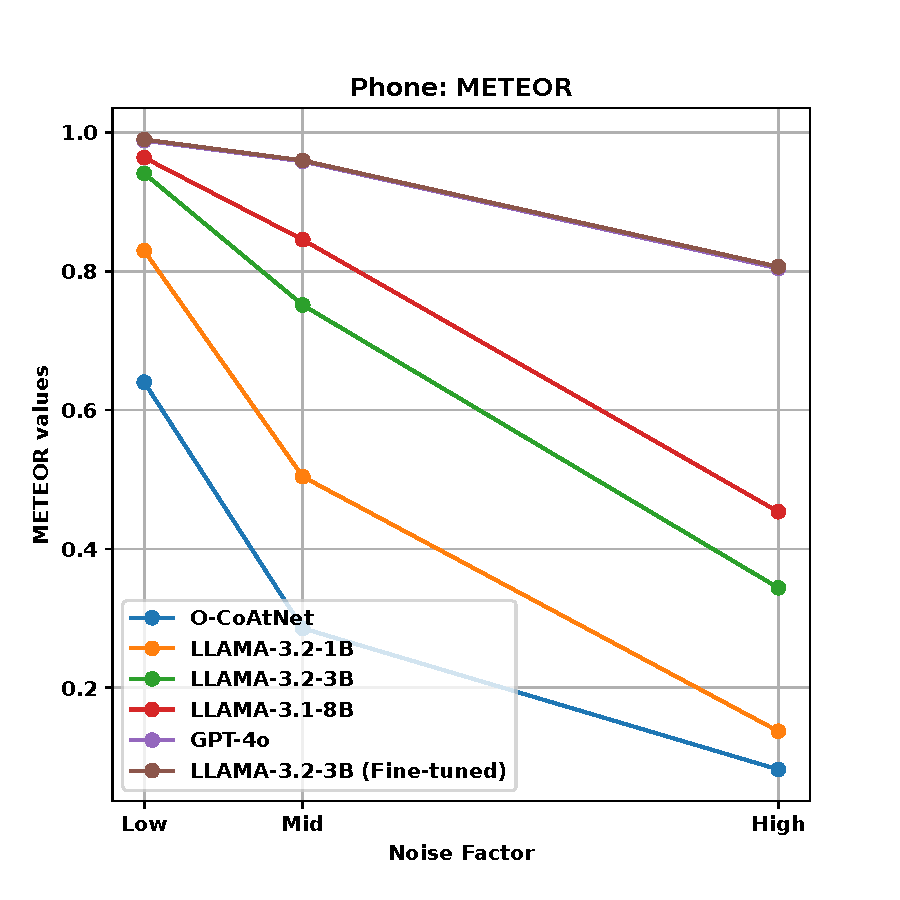
\includegraphics[width=0.20\textwidth]{images/Meteor_Score_phone.pdf}\hfill
    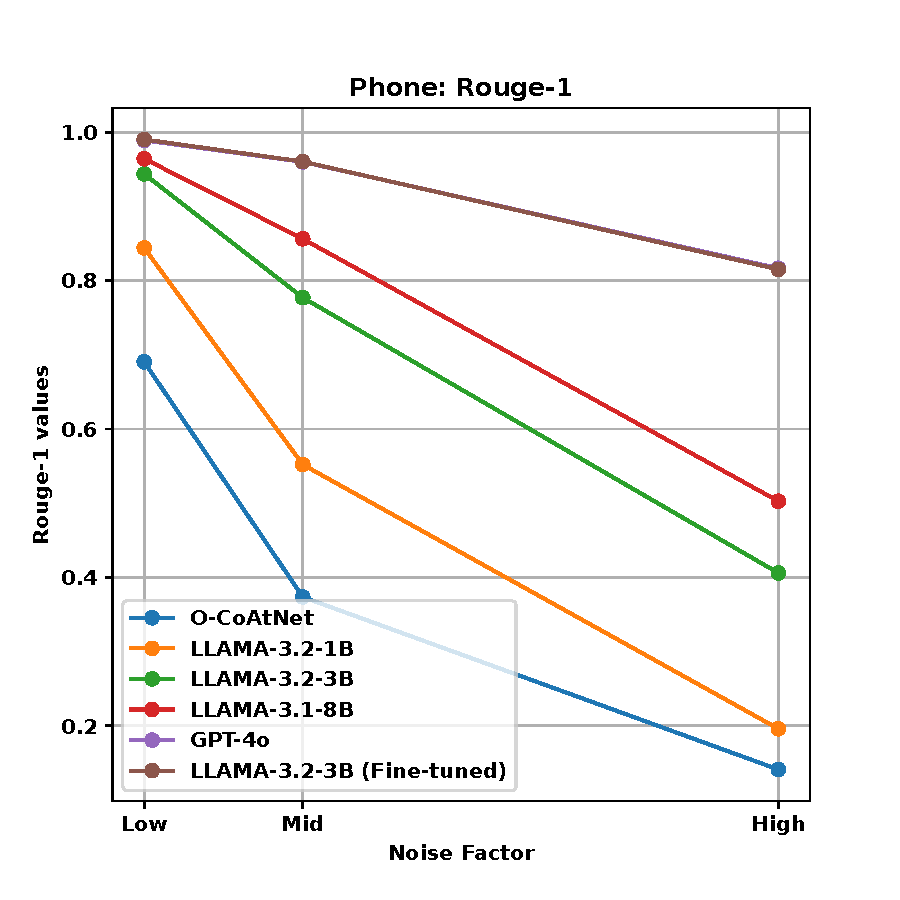
\includegraphics[width=0.20\textwidth]{images/Rouge_1_phone.pdf}\hfill
    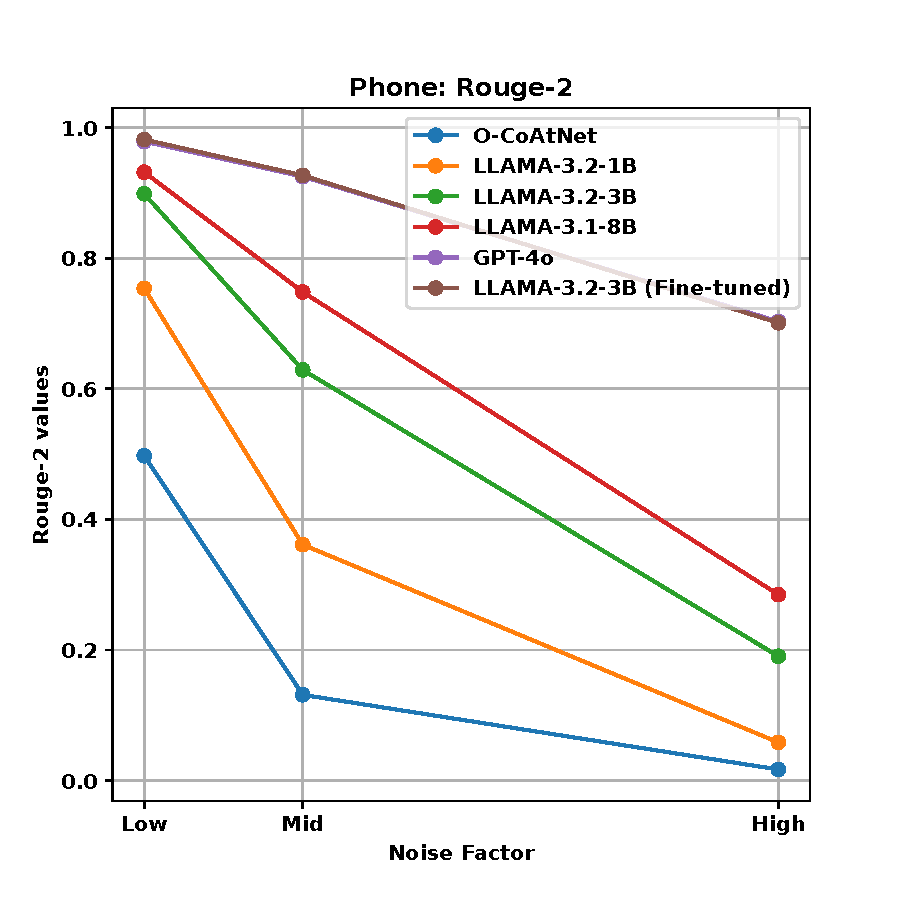
\includegraphics[width=0.20\textwidth]{images/Rouge_2_phone.pdf}\hfill
    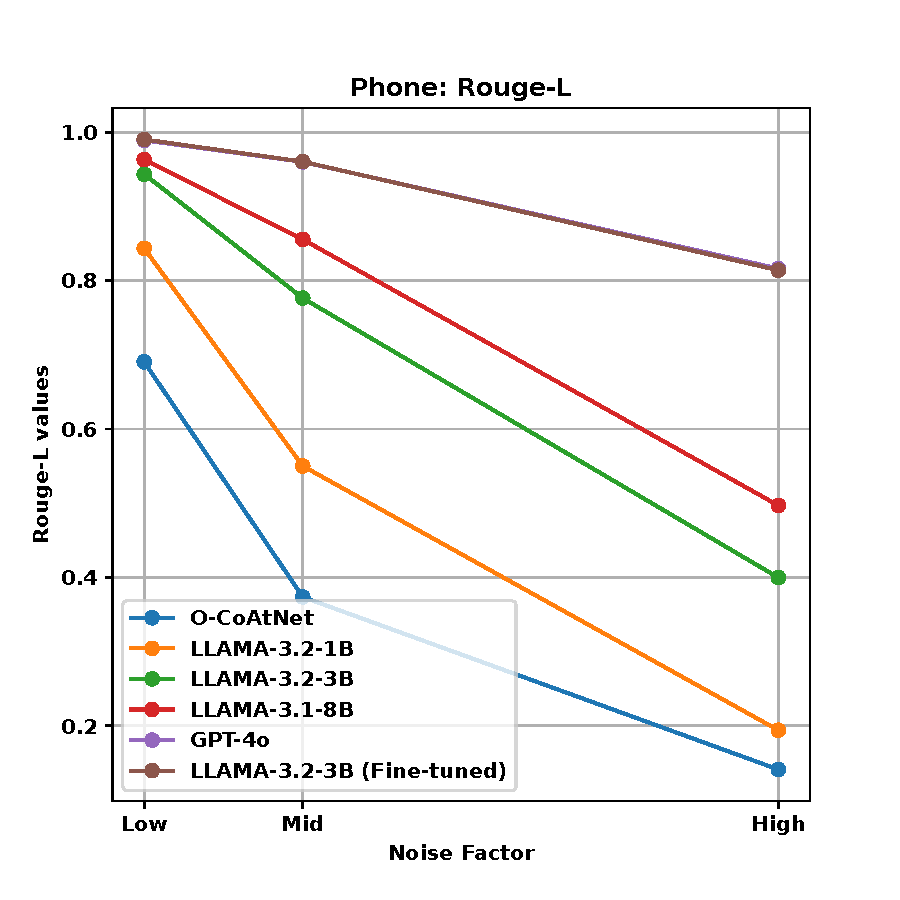
\includegraphics[width=0.20\textwidth]{images/Rouge_L_phone.pdf}\hfill

    % zoom
    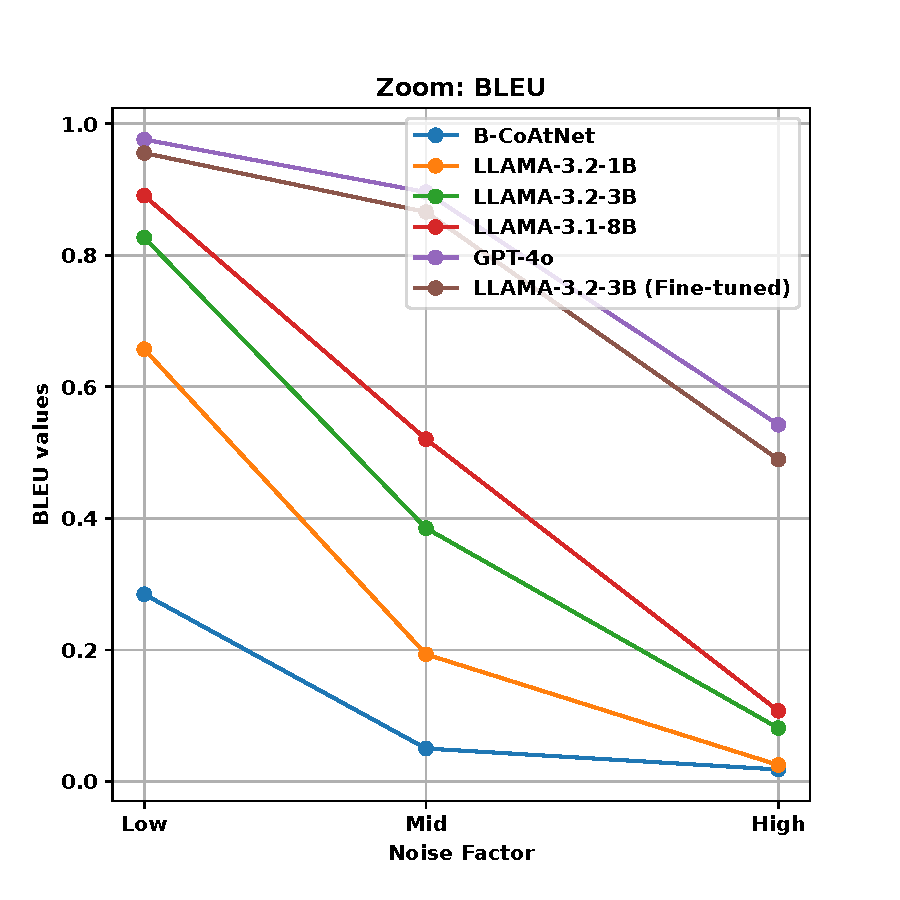
\includegraphics[width=0.20\textwidth]{images/bleu_zoom.pdf}\hfill
    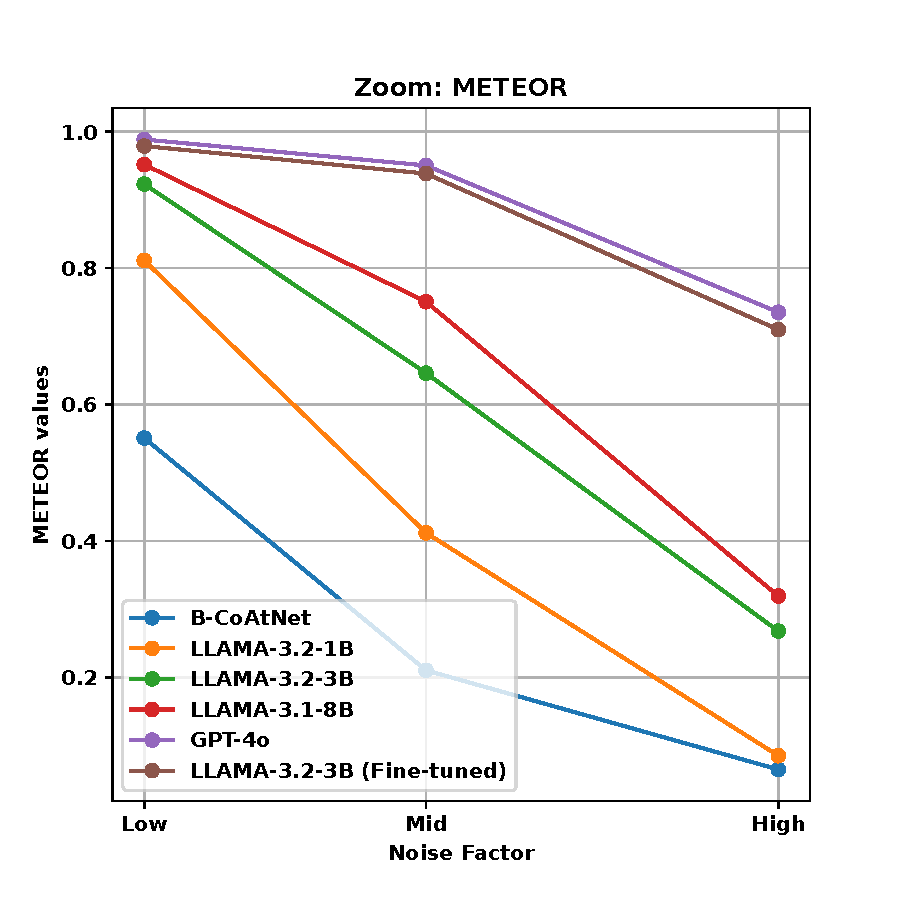
\includegraphics[width=0.20\textwidth]{images/meteor_zoom.pdf}\hfill
    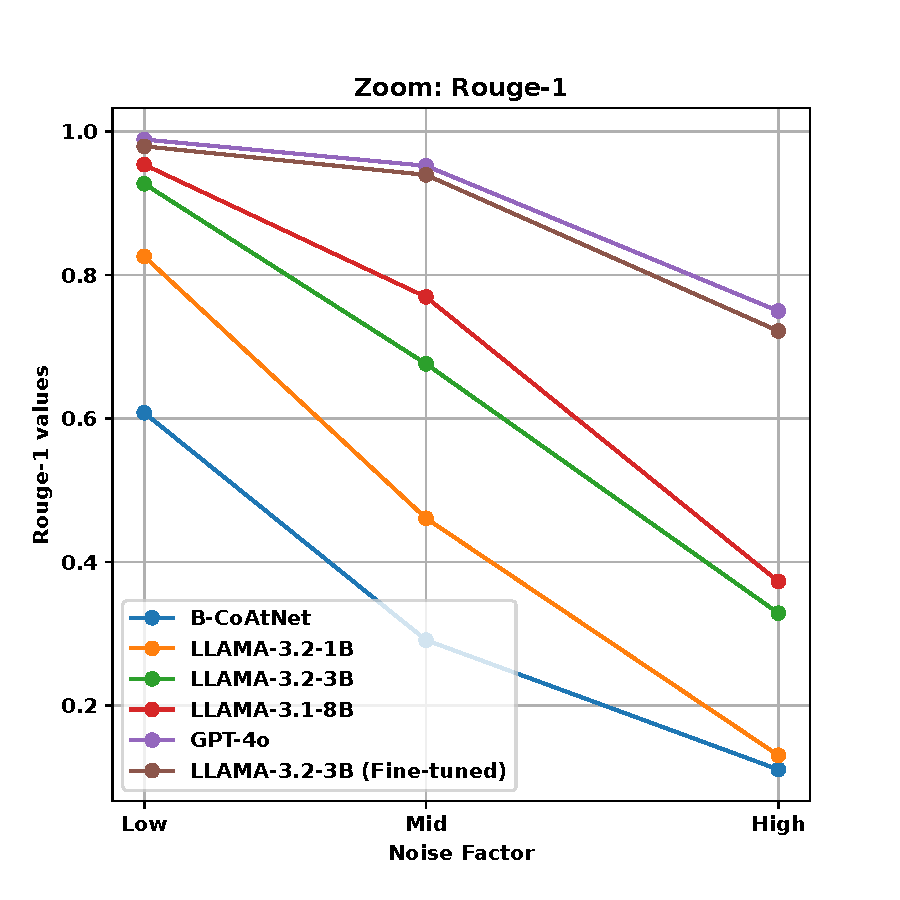
\includegraphics[width=0.20\textwidth]{images/rouge1_zoom.pdf}\hfill
    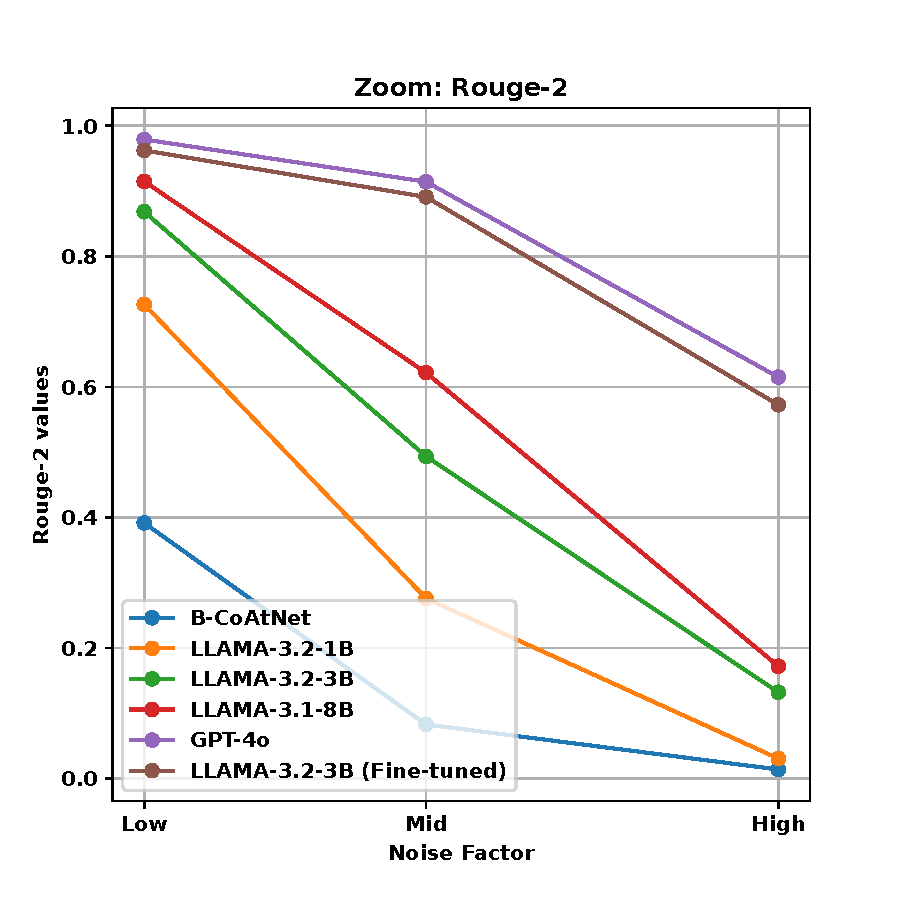
\includegraphics[width=0.20\textwidth]{images/rouge2_zoom.pdf}\hfill
    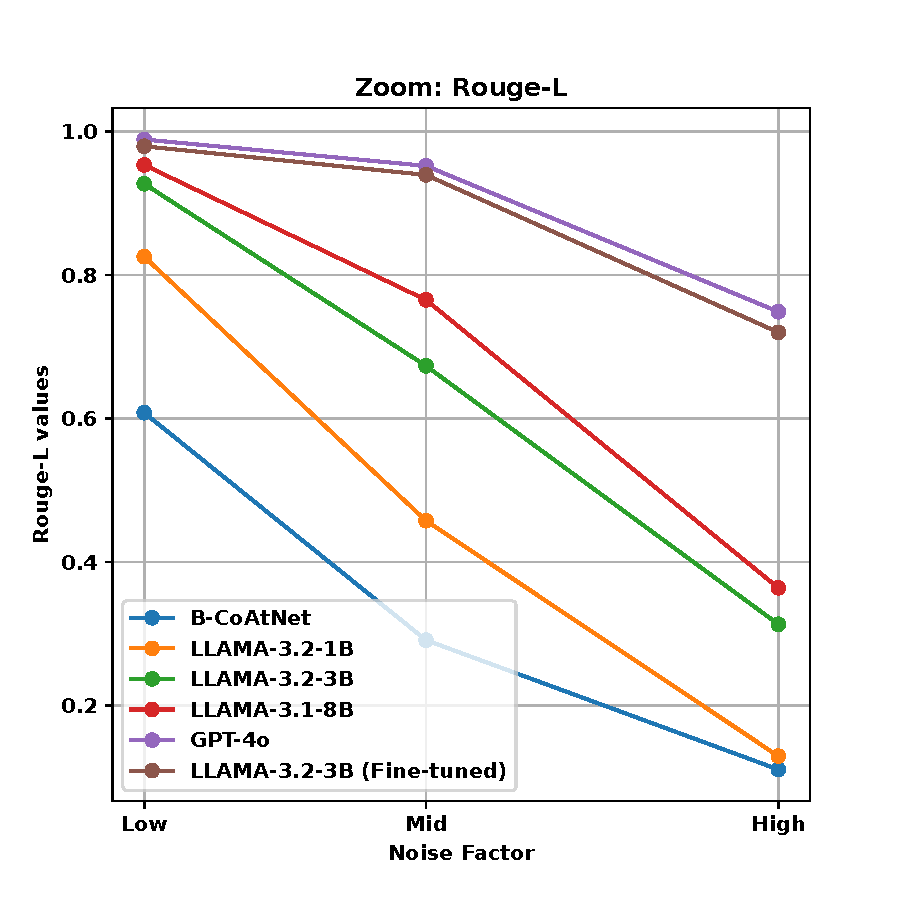
\includegraphics[width=0.20\textwidth]{images/rougeL_zoom.pdf}

    \caption{Performance using metrics -- BLEU, METEOR, ROUGE-1, ROUGE-2, and ROUGE-L -- for different models including the fine-tuned Llama-3.2-3B model at varying noise factors on the Phone and Zoom datasets. For clarity, only the mean is displayed in this graph; the standard deviation is omitted.}
    \label{fig:rotated}
\end{figure*}


% The small size enables our pipeline to be deployed in many more settings. It can be easily stored and computed locally on regular home computers or even mobile devices.

% \todo{to make this paper really strong, we would need to have a case study here to demonstrate the type of information that we can retreive (e.g., passwords). We probably dont have time (or data) to do it, but i leave the suggestion here so if you have time you can think about something}